%% LyX 2.3.4.2 created this file.  For more info, see http://www.lyx.org/.
%% Do not edit unless you really know what you are doing.
\documentclass[english,dvipsnames,aspectratio=169]{beamer}
\usepackage{mathptmx}
\usepackage{eulervm}
\usepackage[T1]{fontenc}
\usepackage[latin9]{inputenc}
\usepackage{babel}
\usepackage{amstext}
\usepackage{amssymb}
\usepackage{graphicx}
\usepackage{ifthen}
\usepackage{xcolor}
\usepackage{xspace}
\usepackage{tikz}
\usetikzlibrary{tikzmark}
\usetikzlibrary{calc}
\usepackage{pgfplots}
%\pgfplotsset{compat=1.17}
\usepackage{booktabs}
\usepackage{xpatch}
\usepackage{multirow}
\usepackage{colortbl}
\usepackage{pgfpages}


\xpatchcmd{\itemize}
  {\def\makelabel}
  {\ifnum\@itemdepth=1\relax
     \setlength\itemsep{2ex}% separation for first level
   \else
     \ifnum\@itemdepth=2\relax
       \setlength\itemsep{1ex}% separation for second level
     \else
       \ifnum\@itemdepth=3\relax
         \setlength\itemsep{0.5ex}% separation for third level
   \fi\fi\fi\def\makelabel
  }
 {}
 {}

\ifx\hypersetup\undefined
  \AtBeginDocument{%
    \hypersetup{unicode=true,pdfusetitle,
 bookmarks=true,bookmarksnumbered=false,bookmarksopen=false,
 breaklinks=false,pdfborder={0 0 0},pdfborderstyle={},backref=false,colorlinks=true,
 allcolors=NYUPurple,urlcolor=LightPurple}
  }
\else
  \hypersetup{unicode=true,pdfusetitle,
 bookmarks=true,bookmarksnumbered=false,bookmarksopen=false,
 breaklinks=false,pdfborder={0 0 0},pdfborderstyle={},backref=false,colorlinks=true,
 allcolors=NYUPurple,urlcolor=LightPurple}
\fi

\makeatletter

%%%%%%%%%%%%%%%%%%%%%%%%%%%%%% LyX specific LaTeX commands.
%% Because html converters don't know tabularnewline
\providecommand{\tabularnewline}{\\}

%%%%%%%%%%%%%%%%%%%%%%%%%%%%%% Textclass specific LaTeX commands.
% this default might be overridden by plain title style
\newcommand\makebeamertitle{\frame{\maketitle}}%
% (ERT) argument for the TOC
\AtBeginDocument{%
  \let\origtableofcontents=\tableofcontents
  \def\tableofcontents{\@ifnextchar[{\origtableofcontents}{\gobbletableofcontents}}
  \def\gobbletableofcontents#1{\origtableofcontents}
}

%%%%%%%%%%%%%%%%%%%%%%%%%%%%%% User specified LaTeX commands.
\usetheme{CambridgeUS} 
\beamertemplatenavigationsymbolsempty


% Set Color ==============================
\definecolor{NYUPurple}{RGB}{87,6,140}
\definecolor{LightPurple}{RGB}{165,11,255}


\setbeamercolor{title}{fg=NYUPurple}
\setbeamercolor{frametitle}{fg=NYUPurple}

\setbeamercolor{background canvas}{fg=NYUPurple, bg=white}
\setbeamercolor{background}{fg=black, bg=NYUPurple}

\setbeamercolor{palette primary}{fg=black, bg=gray!30!white}
\setbeamercolor{palette secondary}{fg=black, bg=gray!20!white}
\setbeamercolor{palette tertiary}{fg=gray!20!white, bg=NYUPurple}

\setbeamertemplate{headline}{}
\setbeamerfont{itemize/enumerate body}{}
\setbeamerfont{itemize/enumerate subbody}{size=\normalsize}

\setbeamercolor{parttitle}{fg=NYUPurple}
\setbeamercolor{sectiontitle}{fg=NYUPurple}
\setbeamercolor{sectionname}{fg=NYUPurple}
\setbeamercolor{section page}{fg=NYUPurple}
%\setbeamercolor{description item}{fg=NYUPurple}
%\setbeamercolor{block title}{fg=NYUPurple}

\setbeamertemplate{blocks}[rounded][shadow=false]
\setbeamercolor{block body}{bg=normal text.bg!90!NYUPurple}
\setbeamercolor{block title}{bg=NYUPurple!30, fg=NYUPurple}



\AtBeginSection[]{
  \begin{frame}
  \vfill
  \centering
\setbeamercolor{section title}{fg=NYUPurple}
 \begin{beamercolorbox}[sep=8pt,center,shadow=true,rounded=true]{title}
    \usebeamerfont{title}\usebeamercolor[fg]{title}\insertsectionhead\par%
  \end{beamercolorbox}
  \vfill
  \end{frame}
}

\makeatother

\setlength{\parskip}{\medskipamount} 

\input ../macros

\begin{document}
\input ../rosenberg-macros

%\setbeameroption{show notes on second screen}

\title[DS-GA 1003]{Decision Trees}
\author{Tal Linzen\\
Slides based on Lecture
\href{https://github.com/davidrosenberg/mlcourse/blob/gh-pages/Lectures/10.trees.pdf}{10} from David Rosenberg's course materials (\url{https://github.com/davidrosenberg/mlcourse})
}
\date{April 5, 2022}
\institute{CDS, NYU}

\makebeamertitle
\mode<article>{Just in article version}

\begin{frame}
{Today's lecture}
\begin{itemize}
\item Our first inherently non-linear classifier: decision trees.
\item Ensemble methods: bagging and boosting.
\end{itemize}
\end{frame}

\section{Decision Trees}

\begin{frame}{Regression trees: Predicting basketball players' salaries}
    \begin{minipage}{0.45\textwidth}
        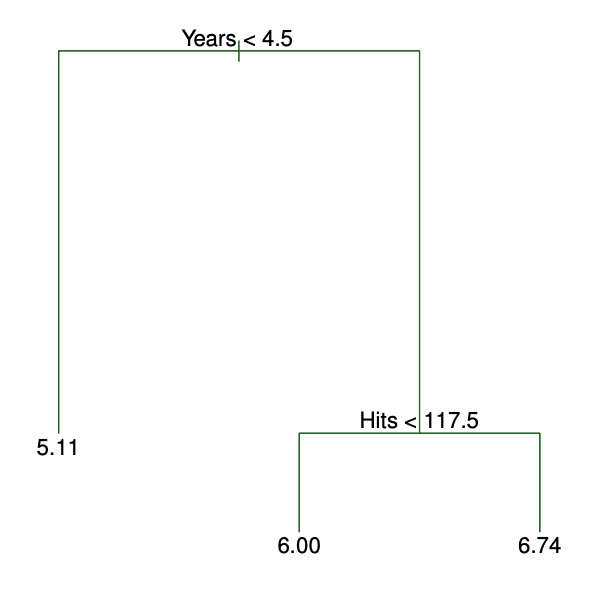
\includegraphics[width=\textwidth]{figures/basketball_decision_tree}
    \end{minipage}%
    \begin{minipage}{0.45\textwidth}
        \pause
        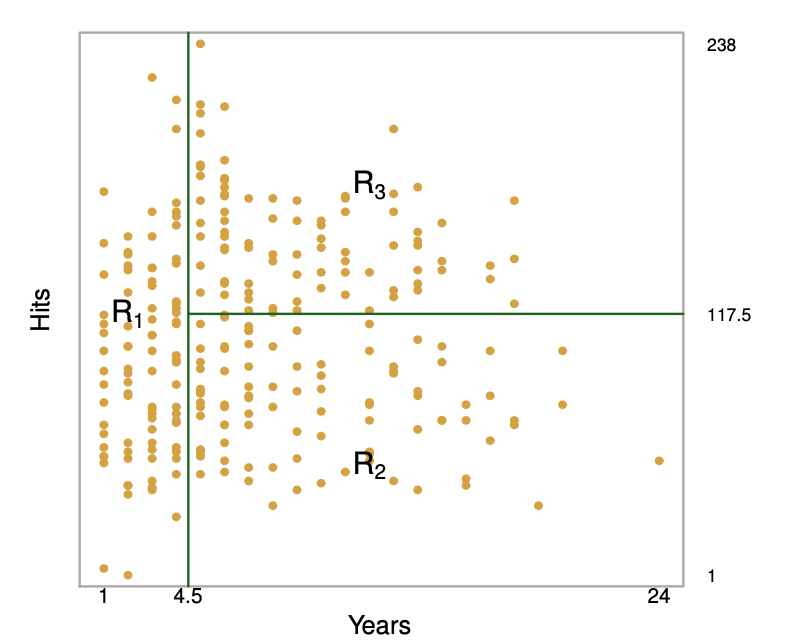
\includegraphics[height=\textwidth]{figures/basketball_regions}
    \end{minipage}
\end{frame}

\begin{frame}
    {Classification trees}
%\item Decision tree is a \textcolor{blue}{non-linear} classifier
\begin{center}
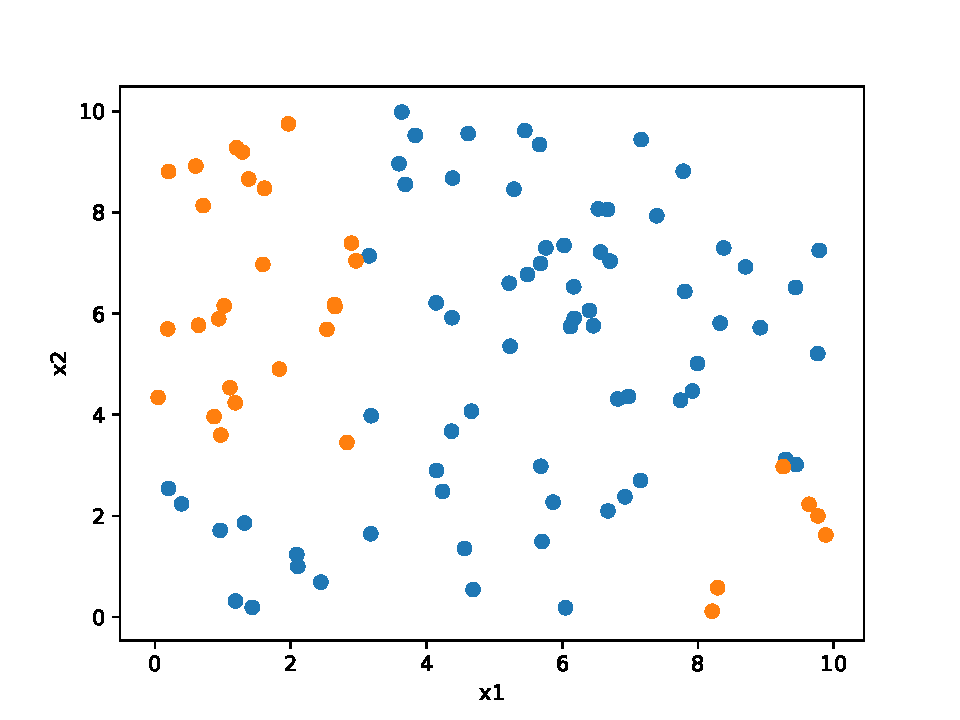
\includegraphics[height=0.6\textheight]{figures/dt-2d}
\end{center}
\begin{itemize}
\item Can we classify these points using a linear classifier?
    \pause
\item Partition the data into axis-aligned regions \textcolor{blue}{recursively} (on the board)
\end{itemize}
\note[item]{Let's consider the dataset shown in the figure. How should we classify the orange and the blue points?}
\note[item]{They are not linearly separable, but they belong to different regions. (draw regions)}
\note[item]{Let's partition the space recursively.}
\end{frame}

\begin{frame}
{Decision trees setup}
\begin{columns}
\begin{column}{0.5\textwidth}
\begin{center}
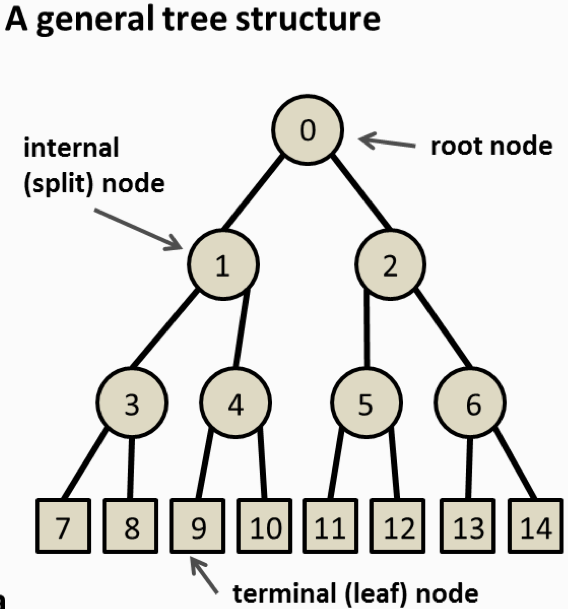
\includegraphics[height=0.7\textheight]{figures/generalTreeStructure}
\end{center}
\note<.>{Explain depth of a tree.}
\end{column}
\begin{column}{0.5\textwidth}
    \begin{itemize}[<+->]
\item We focus on \emph{binary} trees (as opposed to multiway trees where nodes can have more
than two children)
\item Each node contains a subset of data points
\item The data splits created by each node involve only a \emph{single} feature
\item For continuous variables, the splits are always of the form $x_{i}\le t$
\item For discrete variables, we partition values into two sets (not covered today)
\item Predictions are made in terminal nodes
\end{itemize}
\end{column}
\end{columns}
\let\thefootnote\relax\footnotetext{\tiny{From Criminisi et al. MSR-TR-2011-114, 28 October 2011.}}

\note[item]{Let's review some terminology for trees you've probably seen in an algorithm class. We'll consider a rooted tree, where we have a designated root node. The nodes that have degree one (incident to only one edge) are terminal/leaf nodes. The other nodes are called internal nodes.}
\note[item]{Specifically, we'll consider binary trees where each node has two children.}
\note[item]{What does each node represent? They correspond to one partition of the data. The root node contains all data; we partition the data in one node by branching to its descendants.}
\note[item]{The branching decision at each node involves a single feature.}
\end{frame}

   
\begin{frame}
    {Constructing the tree}
\begin{description}[<+->]
        \item[Goal] Find boxes $R_1, \ldots, R_J$ that minimize $\sum\limits_{j=1}^{J}\sum\limits_{i\in R_j} (y_i - \hat y_{R_j})^2$, subject to complexity constraints.
\item[Problem] Finding the optimal binary tree is computationally intractable.
\item[Solution] Greedy algorithm: starting from the root, and repeating until a stopping criterion is reached (\eg max depth), find the non-terminal node that results in the ``best'' split
    \begin{itemize}
        \item We only split regions defined by previous non-terminal nodes
    \end{itemize}
\item[Prediction] Our prediction is the mean value of a terminal node: $\hat y_{R_m} = \text{mean}(y_i \mid x_i \in R_m)$
    \begin{itemize}
\item A greedy algorithm is the one that make the best \textbf{local} decisions, without lookahead to evaluate their downstream consequences
    \item This procedure is not very likely to result in the globally optimal tree
    \end{itemize}
\end{description}
\note[item]{Given some stopping criteria, the next question is how do we find the split that will minimize our task loss in the end.}
\note[item]{In general, this is intractable.}
\note[item]{However, we can use a greedy algorithm to split each node in a locally optimal way, starting from the root.}
\end{frame}


\begin{frame}{Prediction in a Regression Tree}
    \begin{minipage}{0.3\textwidth}
        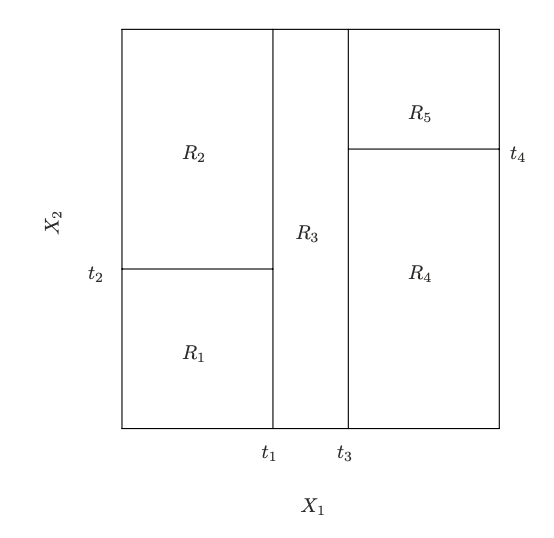
\includegraphics[height=0.5\textheight]{figures/regression_regions}
    \end{minipage}
    \begin{minipage}{0.6\textwidth}
    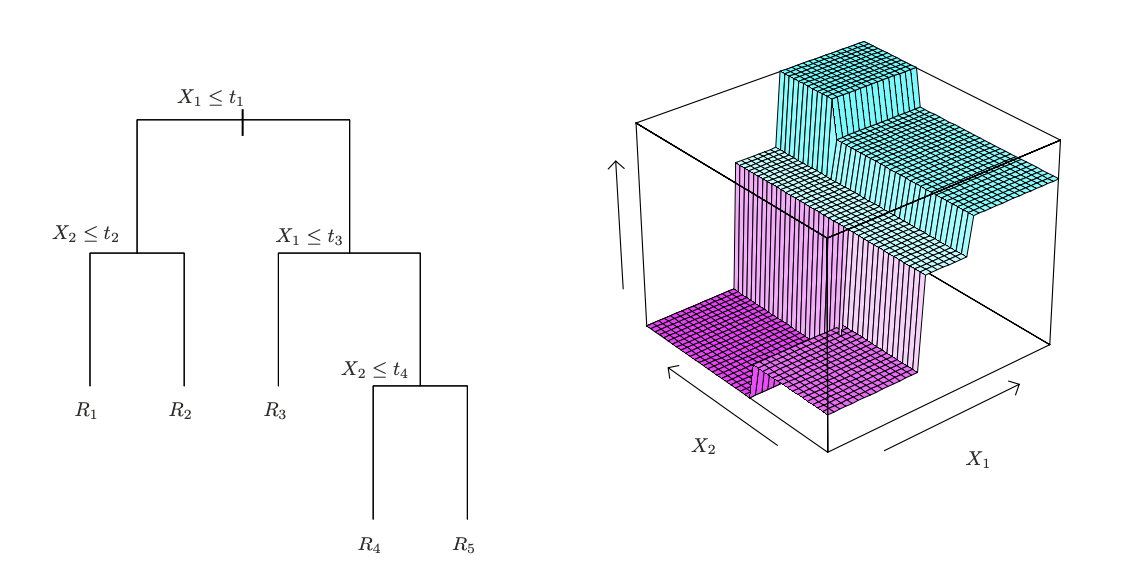
\includegraphics[height=0.6\textheight]{figures/regression_splits_and_surface}
    \end{minipage}
\end{frame}

\begin{frame}{Finding the Best Split Point}
\begin{itemize}[<+->]
\item We enumerate all features and all possible split points for each feature. There are infinitely many split points, but...
\item Suppose we are now considering splitting on the $j$-th feature $x_{j}$, and let $x_{j(1)},\ldots,x_{j(n)}$ be the sorted values of the $j$-th
feature.
\item We only need to consider split points between two adjacent values, and any split point in the interval $(x_{j(r)}, x_{(j(r+1)})$ will result in the same loss 
\item It is common to split half way between two adjacent values:
\begin{align}
s_{j}\in\left\{ \frac{1}{2}\left(x_{j(r)}+x_{j(r+1)}\right)\mid r=1,\ldots,n-1\right\} .
&& \text{$n-1$ splits}
\end{align}
\end{itemize}

\note[item]{Now that we have a measure of goodness for each split. How do we find that split? There are infinitely many split points for each continuous feature.}
\note[item]{But many split points will result in the same regions.}
\end{frame}

\begin{frame}
    {Decision Trees and Overfitting}
\begin{itemize}[<+->]
\item What will happen if we keep splitting the data into more and more regions?
\begin{itemize}
\item Every data point will be in its own region---\textcolor{red}{overfitting}.
\end{itemize}

\item When should we stop splitting? (Controlling the complexity of the hypothesis space)
\begin{itemize}[<.->]
\item Limit total number of nodes.
\item Limit number of terminal nodes.
\item Limit tree depth.
\item Require minimum number of data points in a terminal node.
\item \textbf{Backward pruning} (the approach used in \textbf{CART}; Breiman et al 1984): 
\begin{enumerate}
\item Build a really big tree (e.g. until all regions have $\le5$ points).
\item \emph{Prune} the tree back greedily, potentially all the way to the root,
until validation performance starts decreasing.
\end{enumerate}
\end{itemize}
\end{itemize}
\note[item]{A common approach in practice is backward pruning, similar to backward feature selection. The advantage is that we get the global view once the entire tree is built, where as in the other approaches we might stop too early and miss an important split that only comes later.}
\end{frame}

\begin{frame}{Pruning: Example}
    \centering
    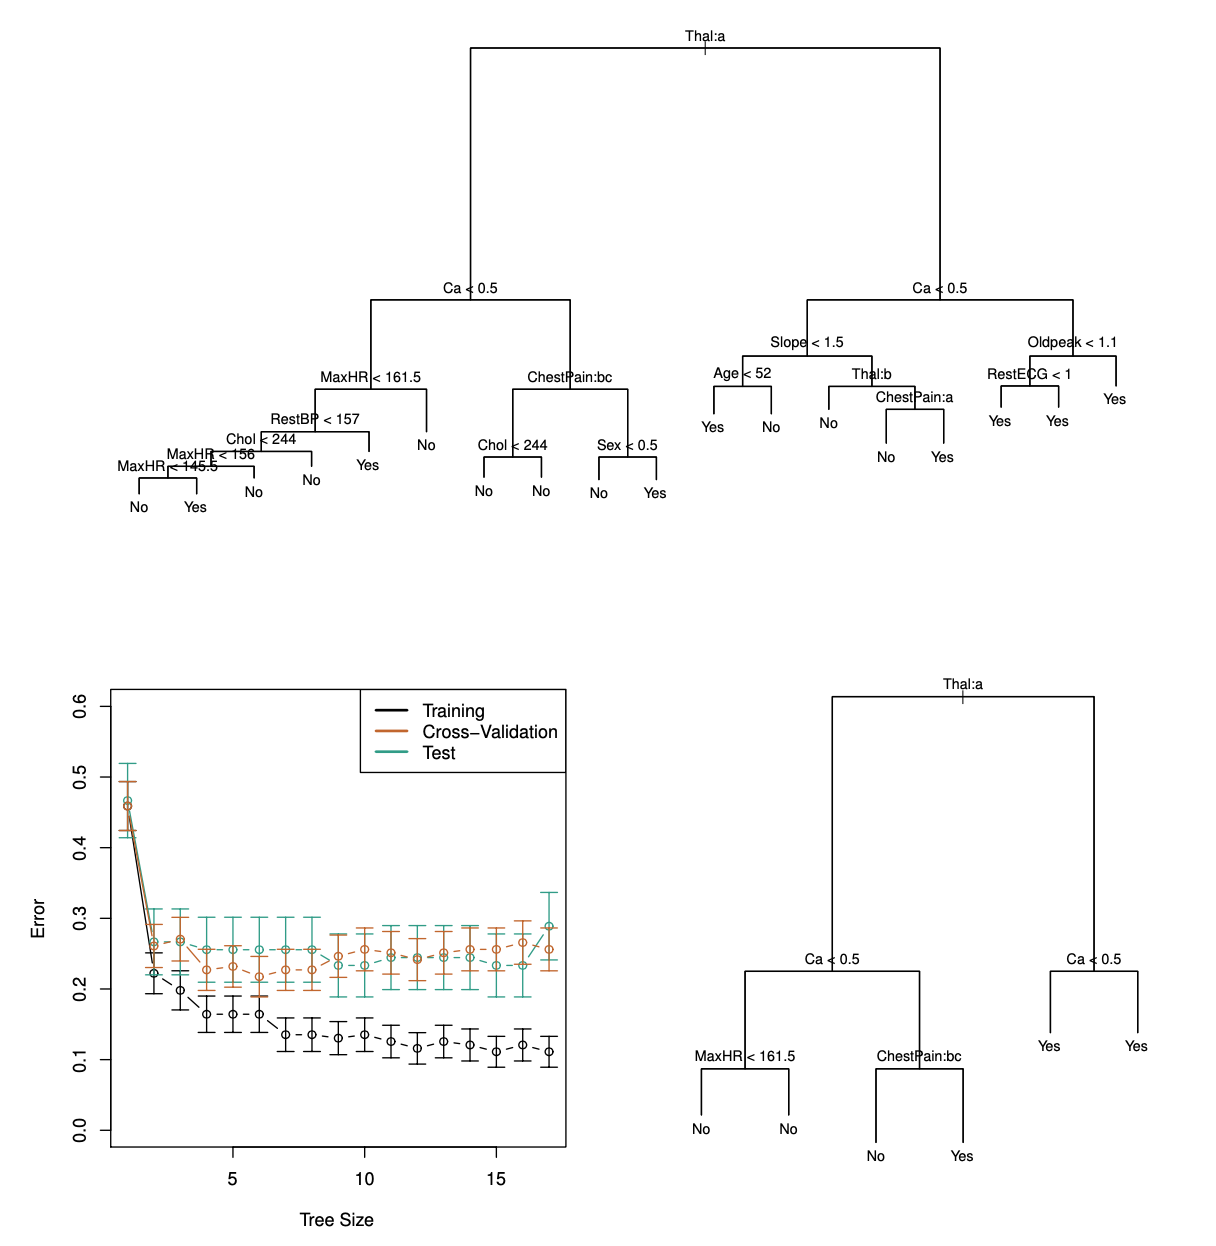
\includegraphics[height=0.8\textheight]{figures/pruning}
\end{frame}

\begin{frame}
{What Makes a Good Split for Classification?}

Our plan is to predict the \textbf{majority label} in each region.
\onslide<+->{
    \begin{simpleblock}{Which of the following splits is better?}
\begin{description}
\item[Split 1] $R_1: 8+ / 2- \qquad R_2: 2+ / 8-$
\item[Split 2] $R_1: 6+ / 4- \qquad R_2: 4+ / 6-$
\end{description}
\end{simpleblock}
}
\onslide<+->{
    \begin{simpleblock}{How about here?}
\begin{description}
\item[Split 1] $R_1: 8+ / 2- \qquad R_2: 2+ / 8-$
\item[Split 2] $R_1: 6+ / 4- \qquad R_2: 0+ / 10-$
\end{description}
\end{simpleblock}
}

\onslide<+->{
Intuition: we want to produce \emph{pure} nodes,
\ie nodes where most instances have the same class.
}
\note[item]{Split 1 is better because it has low error rate.}
\note[item]{It's a bit tricky now. Both split has the same error rate. Note that in Split 2, R2 would be a terminal node already, so we might prefer Split 2; however, R1 still needs more work.}
\end{frame}

\begin{frame}
{Misclassification error in a node}
\begin{itemize}
\item Let's consider the multiclass classification case: $\cy=\left\{ 1,2,\ldots,K\right\} $.

\item Let node $m$ represent region $R_{m}$, with $N_{m}$ observations
\item We denote the proportion of observations in $R_{m}$ with class $k$ by
\[
\hat{p}_{mk}=\frac{1}{N_{m}}\sum_{\left\{ i:x_{i}\in R_{m}\right\} }\ind{y_{i}=k}.
\]

\item We predict the majority class in node $m$: 
    \[ 
        k(m)=\argmax_{k}\hat{p}_{mk} 
    \]

%\item The misclassification rate in node $m$ is $1-\hat{p}_{mk(m)}$
\end{itemize}

\note[item]{Each node contains a subset of data.}
\end{frame}

\begin{frame}{Node Impurity Measures}
\begin{itemize}[<+->]
\item Three measures of \textbf{node impurity} for leaf node
$m$:
\begin{description}[<+->][Misclassification error]
\item[Misclassification error]
\[
1 -  \hat{p}_{mk(m)}.
\]

\item[The Gini index] encourages $\hat{p}_{mk}$ to be close to 0 or 1
\[
\sum_{k=1}^{K}\hat{p}_{mk}(1-\hat{p}_{mk})
\]

\item[Entropy / Information gain]
\[
-\sum_{k=1}^{K}\hat{p}_{mk}\log\hat{p}_{mk}.
\]
\end{description}
\item The Gini index and entropy are numerically similar to each other, and both work better in practice than the misclassification error.

\note[item]{We would like a metric that gives high scores to nodes containing examples from many different classes, and low scores to nodes with few or a single class of examples.}
\note[item]{We've seen that the error rate can indicate node purity. When is it minimized? When $p$ is 1, i.e., all examples are in the same class. Note that this is different from the Gini index that measure inequality you might learn in economics.}
\note[item]{But it's not a ``sensitive'' measure. It's often the case that we will have many splits that gives the same misclassification error. Gini index is another popular metric. For each class $k$ we compute the product of the proportion of class $k$, $\hat{p}_{mk}$ and the other classes $1-\hat{p}_{mk}$. When is it minimized? $p=0 / 1$.}
\note[item]{Finally, we can use Shannon entropy, which measure the uncertainty of the label in this node. It's minimized when all labels are the same---no uncertainty.}
\note[item]{Both Gini index and entropy are information-theoretic measures.}

\end{itemize}
\end{frame}

\begin{frame}{Impurity Measures for Binary Classification}

    \centering
    ($p$ is the relative frequency of class 1)
\begin{figure}
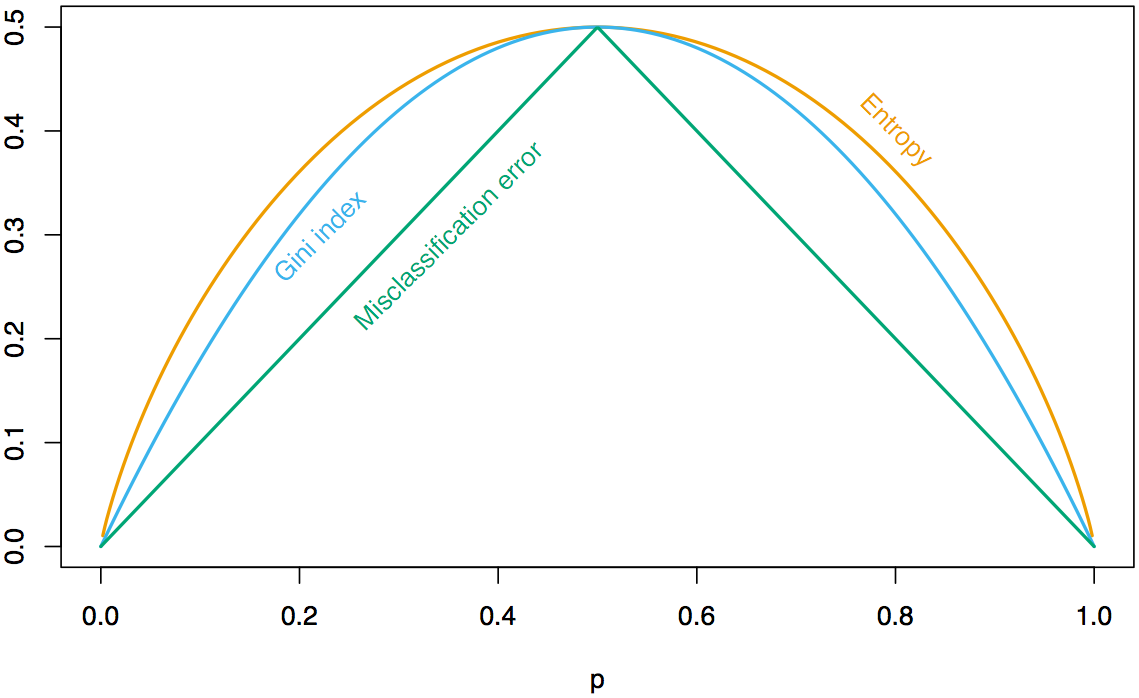
\includegraphics[height=0.5\textheight]{figures/impurityMeasureTwoClass}
\end{figure}
\vspace{-1em}
%Misclassification error is not strictly concave thus may not guarantee improvement over the parent node.
\note[item]{On the linear piece of misclassification error,
$w_1Q(p_1) + w_2Q(p_2) = Q(w_1p_1 + w_2p_2)$.}
\let\thefootnote\relax\footnotetext{\tiny{HTF Figure 9.3}}
\end{frame}

\begin{frame}{Quantifying the Impurity of a Split}
Scoring a potential split that produces the nodes $R_{L}$ and $R_{R}$:
\begin{itemize}
\item Suppose we have $N_{L}$ points in $R_{L}$ and $N_{R}$ points in
$R_{R}$.

\item Let $Q(R_{L})$ and $Q(R_{R})$ be the node impurity measures for each node.

\item We aim to find a split that minimizes the \emph{weighted average of node
impurities}:
\[
\frac{N_{L}Q(R_{L})+N_{R}Q(R_{R})}{N_L+N_R}
\]
\end{itemize}

\note[item]{Now that we've defined impurity measure for a single node, how do we use it to evaluate a split, which produces two nodes?}
\note[item]{The weight is just the proportion of examples in left and right nodes.}
\note[item]{$Q_1 = 1/4, Q_2=1/4, w_1 = 10/15=2/3, w_2 = 1/3.$}
\end{frame}


%\begin{frame}
%{Regression trees}
%\begin{itemize}
%\item Squared loss as the node impurity measure.
%%\item Everything else remains the same as classification trees.
%\end{itemize}

%\note[item]{How do we apply the same splitting strategy for regression problems? What needs to be changed?}
%\note[item]{First, instead of predicting the majority class, we predict the mean.}
%\note[item]{Impurity is easier---just squared loss, i.e. how much the values deviate from the mean.}
%\note[item]{So, to recap, to grow a basic decision tree, we pick an impurity measure and a stopping criterion, start from the root node, then recursively split until a stop criteria is reached. Next, let's consider some practical matters.}
%\end{frame}

%\subsection{Trees in General}
%\begin{frame}
%{\dis Categorical features}
%\begin{itemize}[<+->]
%\item For a categorical feature, we split its values into two groups.
%\item<.-> Given a set of categories of size $k$, how many distinct splits? (its power set)
%\item Finding the optimal split is \textcolor{red}{intractable} in general.
%\item Approximations
%\begin{description}[<.->][Numeric encoding]
%\item<+->[Numeric encoding] Randomly assign a number to each category
%\begin{itemize}
%\item Binary classification: proportion of class 0
%\item Regression: mean of targets of examples in the category, \ie  \textbf{mean encoding} 
%\end{itemize}
%\item[One-hot encoding] May grow imbalanced trees, \eg left-branching
%\item[Binary encoding] Robust to large cardinality
%\end{description}

%\item Statistical issues with categorical features
%\begin{itemize}[<.->]
%\item If a category has a very large number of categories, we can \al{overfit}.
%\item Extreme example: Row Number could lead to perfect classification with
%a single split.
%\end{itemize}
%\end{itemize}
%\note[item]{One unique characteristic of tree-based models is that they handle categorical features naturally.}
%\note[item]{$2^k$ subsets, divided by 2 for symmetry, minus 1 to remove the empty set}
%\note[item]{Approximation: we can either reduce it to the continuous case, or reduce the number of categories.
%To reduce it to the continuous case, we can randomly assign a number to each category. In binary classification, we can do it slightly smartly by assigning the proportion of negative examples in that category.
%To reduce the number of categories, we can use binary encoding, which creates multiple binary features out of one categorical features.}
%\note[item]{We should be careful with overfitting with there are a large number of categories though.}
%\end{frame}

\begin{frame}
{Discussion: Interpretability of Decision Trees}

    \centering
        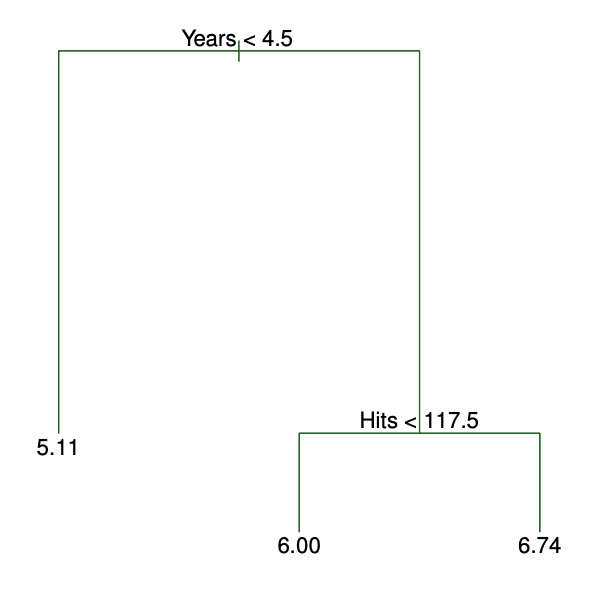
\includegraphics[width=0.2\textwidth]{figures/basketball_decision_tree}
    \begin{itemize}[<+->]
    \item Trees are easier to visualize and explain than other classifiers (even linear regression)
\item Small trees are interpretable -- large trees, maybe not so much
%\item Approximate neural network decision boundaries to gain interpretability
%\begin{itemize}
%\item Wu M, Hughes M, Parbhoo S, Zazzi M, Roth V, Doshi-Velez F. \href{https://finale.seas.harvard.edu/files/finale/files/beyond_sparcity_tree_regularization_of_deep_01.pdf}{Beyond Sparsity: Tree Regularization of Deep Models for Interpretability}. Association for the Advancement of Artificial Intelligence (AAAI). 2018
%\end{itemize}
\end{itemize}
\end{frame}

\begin{frame}
{Discussion: Trees vs. Linear Models}
Trees may have to work hard to capture linear decision boundaries, but can easily capture certain nonlinear ones:
\begin{figure}
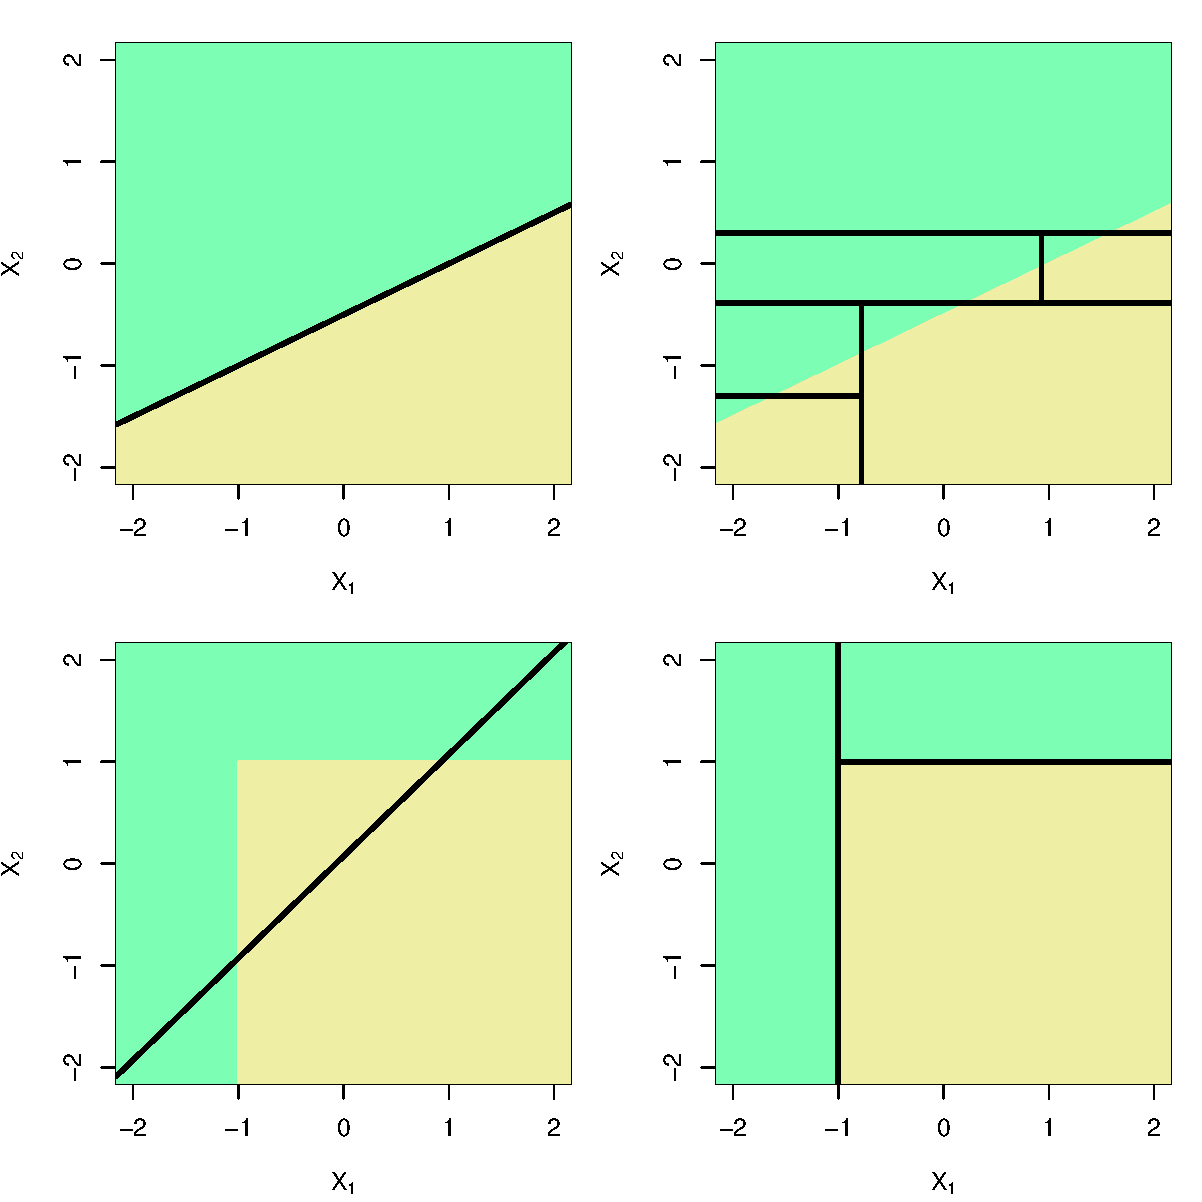
\includegraphics[height=0.6\textheight]{figures/treeVsLinear}
\end{figure}
\note[item]{Because it's hard of it to model the addition of two features.}
\end{frame}

\begin{frame}
{Discussion: Review}
\begin{simpleblock}{Decision trees are:}
\begin{itemize}
\item Non-linear: the decision boundary that results from splitting may end up being quite complicated
\item Non-metric: they do not rely on the geometry of the space (inner products or distances)
\item Non-parametric: they make no assumptions about the distribution of the data
\end{itemize}
\end{simpleblock}

\pause
\begin{simpleblock}{Additional pros:}
\begin{itemize}
\item Interpretable and simple to understand
\end{itemize}
\end{simpleblock}

\pause
\begin{simpleblock}{Cons:}
\begin{itemize}
\item Struggle to capture linear decision boundaries
\item They have high variance and tend to \al{overfit}: they are sensitive to small changes in the training data (The ensemble techniques we discuss next can mitigate these issues)
\end{itemize}
\end{simpleblock}

\note[item]{What are some pros and cons of trees?}
\note[item]{One big issue with trees is that they are very unstable, meaning that if the training data is changed slightly, our classifier will be quite different, and this makes the performance of a single tree not competitive.}
\end{frame}

\section{Bagging and Random Forests}
\subsection{Variance of an Estimator}
\begin{frame}
{Recap: Statistics and Point Estimators}
    \begin{itemize}[<+->]
\item We observe data $\cd=\left(x_{1},x_{2},\ldots,x_{n}\right)$ sampled i.i.d. from a parametric distribution $p(\cdot\mid \theta)$

\item A \textbf{statistic} $s=s(\cd)$ is any function of the data:
\begin{itemize}
\item E.g., sample mean, sample variance, histogram, empirical data distribution
\end{itemize}

\item A statistic $\hat{\theta}=\hat{\theta}(\cd)$ is a \textbf{point estimator}
of $\theta$ if $\hat{\theta}\approx\theta$
\end{itemize}

%\onslide<+->{
%\begin{block}{Review questions}
%In frequentist statistics,
%\begin{itemize}
%\item Is $\theta$ random?
%\item Is $\hat{\theta}$ random?
%\item Is the function $s(\cdot)$ random?
%\end{itemize}
%\end{block}
%}

\note[item]{When we say trees are not stable or have high variance, what do we mean by that precisely? Let's recall properties of point estimators we talked about in frequentist statistics.}
\note[item]{We call a statistic a point estimator if it approximates some unknown parameter.}
\note[item]{The function $s$ is not random, but we plug in random samples of data.}
\end{frame}

\begin{frame}
{Recap: Bias and Variance of an Estimator}
\begin{itemize}[<.->]
    \setlength\itemsep{2pt}
\item Statistics are random, so they have probability distributions.
\item The distribution of a statistic is called a \textbf{sampling distribution}. 
\item<+-> The standard deviation of the sampling distribution is called the \textbf{standard error}.
\item<+-> Some parameters of the sampling distribution we might be interested in:
\begin{description}
\item[Bias]  $\mbox{Bias}(\hat{\theta})\eqdef \ex\pb{\hat{\theta}}-\theta$.
\item[Variance] $\mbox{Var}(\hat{\theta})\eqdef \ex\pb{\hat{\theta}^{2}} - \ex^2\pb{\hat{\theta}}$.
\end{description}
%\item<+-> \dis Is bias and variance random?
%\begin{itemize}
    \note[item]{Neither bias nor variance depend on a specific sample $\cd_{n}$.
        We are \emph{taking expectation over $\cd$.}}
%\end{itemize}
\item<+-> Why does variance matter if an estimator is unbiased?
%\begin{itemize}
    \note[item]{$\hat{\theta}(\sD) = x_1$ is an unbiased estimator of the mean of a Gaussian, but would be farther away from $\theta$ than the sample mean.}
%\end{itemize}
\end{itemize}
\note[item]{Next let's look at how we can reduce variance of an estimator.}
\end{frame}

\subsection{The Benefits of Averaging}
\begin{frame}
{Variance of a Mean}
\begin{itemize}
\item Let $\hat{\theta}(\sD)$ be an unbiased estimator with variance $\sigma^2$:
$\BE\pb{\hat{\theta}} = \theta$, $\mbox{Var}(\hat{\theta}) = \sigma^2$.
\item<+-> So far we have used a single statistic $\hat{\theta} = \hat{\theta}(\sD)$ to estimate $\theta$.
\item<+-> Its standard error is $\sqrt{\mbox{Var}(\hat{\theta})} = \sigma$
\end{itemize}

\onslide<+->{
\begin{itemize}
\item Consider a new estimator that takes the average of i.i.d. $\hat{\theta}_1, \ldots, \hat{\theta}_n$ where $\hat{\theta}_i = \hat{\theta}(\sD^{i})$.
    \pause
\item The average has the same expected value but smaller standard error (recall that $Var(cX) = c^2 Var(X)$, and that the $\hat{\theta}_i$-s are uncorrelated):
\begin{align}
\BE\pb{\frac{1}{n}\sum_{i=1}^n \hat{\theta}_i} = \theta \qquad
\mbox{Var}\pb{\frac{1}{n}\sum_{i=1}^n \hat{\theta}_i} = \frac{\sigma^2}{n}
\label{eqn:variance-of-sample-mean}
\end{align}
\end{itemize}
}
\note[item]{Let's say we want to estimate some parameter $\theta$.}
\note[item]{What is the standard error?}
\note[item]{Now let's consider a new estimator that takes the average of $n$ i.i.d. estimates, each computed from some data $\sD^i$.}
\note[item]{It will still be unbiased, but now the variance is reduced. Try to prove it yourself.}
\end{frame}

\begin{frame}{Averaging Independent Prediction Functions }
    \begin{itemize}[<+->]
\item Suppose we have $B$ independent training sets, all drawn from the same distribution ($\sD \sim p(\cdot\mid \theta)$).

\item Our learning algorithm gives us $B$ prediction functions: $\hat{f}_{1}(x),\hat{f}_{2}(x),\ldots,\hat{f}_{B}(x)$

\item We will define the average prediction function as:
\begin{align}
\hat{f}_{\text{avg}}\eqdef \frac{1}{B}\sum_{b=1}^{B}\hat{f}_{b}
\end{align}

%\item<+-> \dis What's random here?
%\begin{itemize}
    \note[item]{The $B$ independent training sets are random, which gives rise to
        variation among the $\hat{f}_{b}$'s.}
%\end{itemize}

%\item<+-> \think{Concept check}: What's the distribution of $\hat{f}$ called?
%What do we know about the distribution?
\end{itemize}

\note[item]{Concept check: sampling distribution. We don't know anything about it because we don't know the data generating distribution.}
\end{frame}

%
\begin{frame}{Averaging Reduces Variance of Predictions}
\begin{itemize}
\item The average prediction for $x_{0}$ is
\[
\hat{f}_{\text{avg}}(x_{0})=\frac{1}{B}\sum_{b=1}^{B}\hat{f}_{b}(x_{0}).
\]

\item $\hat{f}_{\text{avg}}(x_{0})$ and $\hat{f}_{b}(x_{0})$ have the
same expected value, but

\item $\hat{f}_{\text{avg}}(x_{0})$ has smaller variance:% (see \ref{eqn:variance-of-sample-mean}):
\begin{eqnarray*}
\mbox{\ensuremath{\var}}(\hat{f}_{\mbox{avg}}(x_{0})) = 
\frac{1}{B}\var\left(\hat{f}_{1}(x_{0})\right)
\end{eqnarray*}
\pause
\item \al{Problem}: in practice we don't have $B$ independent training sets!
\end{itemize}
\note[item]{The average prediction has the same expected value as the single prediction, but it has smaller variance.}
\note[item]{But are we done? Just train $n$ predictors and average them?}
\end{frame}

\subsection{Bootstrap}

\begin{frame}{The Bootstrap Sample}
\begin{simpleblock}
{How do we simulate multiple samples when we only have one?}
\begin{itemize}[<+->]
\item A \textbf{bootstrap sample} from $\cd_{n}=\left(x_{1},\ldots,x_{n}\right)$
is a sample of size $n$ drawn \emph{with replacement} from $\cd_{n}$

\item Some elements of $\cd_{n}$ 
will show up multiple times, and
some won't show up at all 
\end{itemize}
\end{simpleblock}

%\onslide<+->{\dis How similar are the bootstrap samples?}
\begin{itemize}[<+->]
\item Each $x_{i}$ has a probability of $(1-1/n)^{n}$ of not being
included in a given bootstrap sample

\item For large $n$,
\begin{align}
\left(1-\frac{1}{n}\right)^{n}\approx\frac{1}{e}\approx.368.
\end{align}

\item<.-> So we expect \textasciitilde 63.2\% of elements of $\cd_n$ will show
up at least once.
\end{itemize}

\note[item]{Now the question is how similar these bootstrap samples are. If they are pretty much the same, its distribution would be far from the actual data generating distribution.}
\note[item]{Because we are sampling with replacement, each element has $1/n$ probability to be selected during each draw. And after $n$ draws, the probability that it's still not selected is $1-1/n$ to the power of $n$.}
\note[item]{Actually $n$ doesn't have to be very large, with $n=1000$, we already reach this number here.}
\note[item]{Since about 60 percent examples shown in each bootstrap sample, they should be fairly different.}
\end{frame}
%
%
\begin{frame}{The Bootstrap Method}
\begin{definition}
A \textbf{bootstrap method } simulates $B$
independent samples from $P$ by taking $B$ bootstrap samples from
the sample $\cd_{n}$.

\end{definition}

\begin{itemize}
\item Given original data $\cd_{n}$, compute $B$ bootstrap samples $D_{n}^{1},\ldots,D_{n}^{B}$.

\item For each bootstrap sample, compute some function
\[
\phi(D_{n}^{1}),\ldots,\phi(D_{n}^{B})
\]

\item Use these values as though $D_{n}^{1},\ldots,D_{n}^{B}$ were
i.i.d. samples from $P$.

\item This often ends up being very close to what we'd get with independent samples from $P$!
\end{itemize}
\end{frame}
%
\begin{frame}{Independent Samples vs. Bootstrap Samples}
\begin{itemize}
\item Point estimator $\hat{\alpha}=\hat{\alpha}(\cd_{100})$ for samples
of size $100$, for a synthetic case where the data generating distribution is known

\item Histograms of $\hat{\alpha}$ based on
\begin{itemize}
    \item 1000 independent samples of size 100 (left), vs.
    \item 1000 bootstrap samples of size 100 (right)

\end{itemize}
\end{itemize}
\begin{figure}
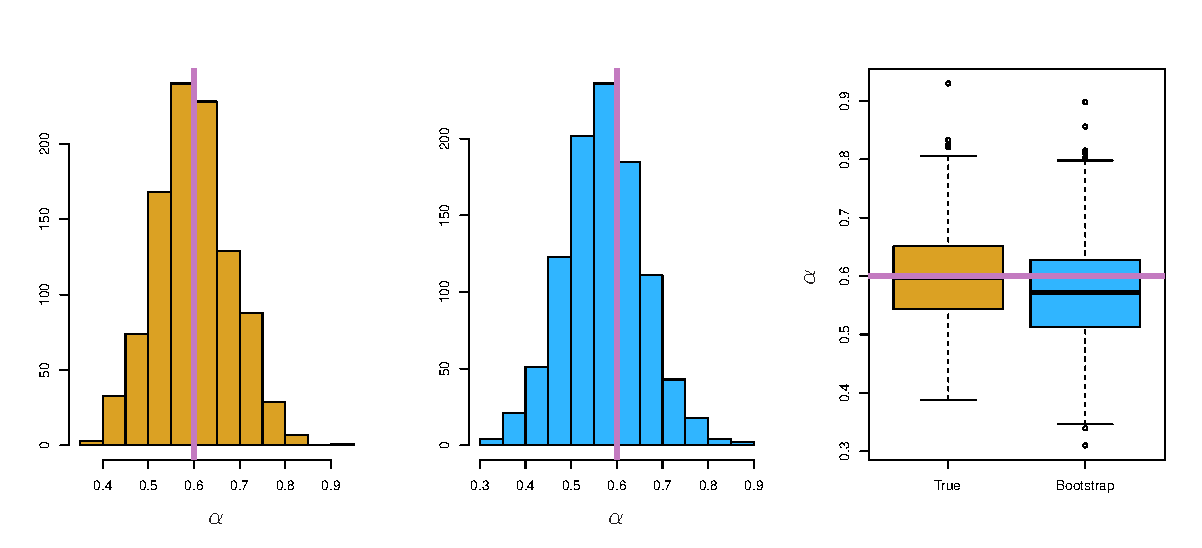
\includegraphics[height=0.4\textheight]{figures/independentVsBootstrap}

\end{figure}

\let\thefootnote\relax\footnotetext{\tiny{Figure 5.10 from \emph{ISLR} (Springer, 2013) with permission from the authors: G. James, D. Witten,  T. Hastie and R. Tibshirani.}}
\end{frame}
%
%\begin{frame}{Side note: Bootstrap in Practice}
%We can use bootstrap to get error bars in a cheap way.
%\begin{itemize}
%\item Suppose we have an estimator $\hat{\theta}=\hat{\theta}(\cd_{n})$.

%\item To get error bars, we can compute the ``\emph{bootstrap variance}''. 

%\begin{itemize}

%\item Draw $B$ bootstrap samples.
%\item Compute sample variance of $\hat{\theta}(\cd_{n}^{1}),\ldots,\hat{\theta}(\cd_{n}^{B})$..

%\item Could report 
%\[
%\hat{\theta}(\cd_{n})\pm\sqrt{\mbox{Bootstrap Variance}}
%\]

%\end{itemize}
%\end{itemize}
%\end{frame}

\begin{frame}{Ensemble Methods}

{\textbf{Key ideas:}}

    \begin{itemize}[<+->]
    \item In general, \textbf{ensemble methods} combine multiple weak models into a single, more powerful model
    \item Averaging i.i.d. estimates reduces variance without changing bias
    \item We can use bootstrap to simulate multiple data samples and average them
    \item Parallel ensemble (\eg bagging): models are built independently
    \item Sequential ensemble (\eg boosting): models are built sequentially
        \begin{itemize}
        \item We try to find new learners that do well where previous learners fall short
        \end{itemize}
\end{itemize}

\end{frame}

\subsection{Bagging}
\begin{frame}{Bagging: Bootstrap Aggregation}
    \begin{itemize}[<+->]
\item We draw $B$ bootstrap samples $D^{1},\ldots,D^{B}$ from original data
$\cd$

\item Let $\hat{f}_{1},\hat{f}_{2},\ldots,\hat{f}_{B}$ be the prediction
functions resulting from training on $D^{1},\ldots,D^{B}$, respectively

\item The \textbf{bagged prediction function} is a \emph{combination }of
these:
\[
\hat{f}_{\text{avg}}(x)=\mbox{Combine}\left(\hat{f}_{1}(x),\hat{f}_{2}(x),\ldots,\hat{f}_{B}(x)\right)
\]

%\pause{}
%\item \dis How might we combine 
%\begin{itemize}
%\item prediction functions for regression?
%\item binary class predictions? 
%\item binary probability predictions?
%\item multiclass predictions? 
%\end{itemize}

    \end{itemize}
\end{frame}

\begin{frame}{Bagging: Bootstrap Aggregation}
    \begin{itemize}[<+->]

\item Bagging is a general method for variance reduction, but it is particularly useful for decision trees

\item For classification, averaging doesn't make sense; we can take a \textbf{majority vote} instead

\item Increasing the number of trees we use in bagging does not lead to overfitting

\item Is there a downside, compared to having a single decision tree?

\item Yes: if we have many trees, the bagged predictor is much less interpretable

\end{itemize}
\end{frame}

\begin{frame}{Aside: Out-of-Bag Error Estimation}
\begin{itemize}
\item Recall that each bagged predictor was trained on about 63\% of the data.
\item The remaining 37\% are called \textbf{out-of-bag (OOB)} observations.

\pause{}
\item For $i$th training point, let 
\[
S_{i}=\left\{ b\mid D^{b}\text{ does not contain }i\text{th point}\right\} 
\]

\item The \textbf{OOB prediction} on $x_{i}$ is
\[
\hat{f}_{\text{OOB}}(x_{i})=\frac{1}{\left|S_{i}\right|}\sum_{b\in S_{i}}\hat{f}_{b}(x_{i})
\]

\item The OOB error is a good estimate of the test error

\item Similar to cross validation error: both are computed
on the training set
\end{itemize}
\end{frame}

\begin{frame}{Applying Bagging to Classification Trees}
\begin{itemize}
\item Input space $\cx=\reals^{5}$ and output space $\cy=\left\{ -1,1\right\} $.
Sample size $n=30$.
\begin{columns}[t]

\column{.4\textwidth}

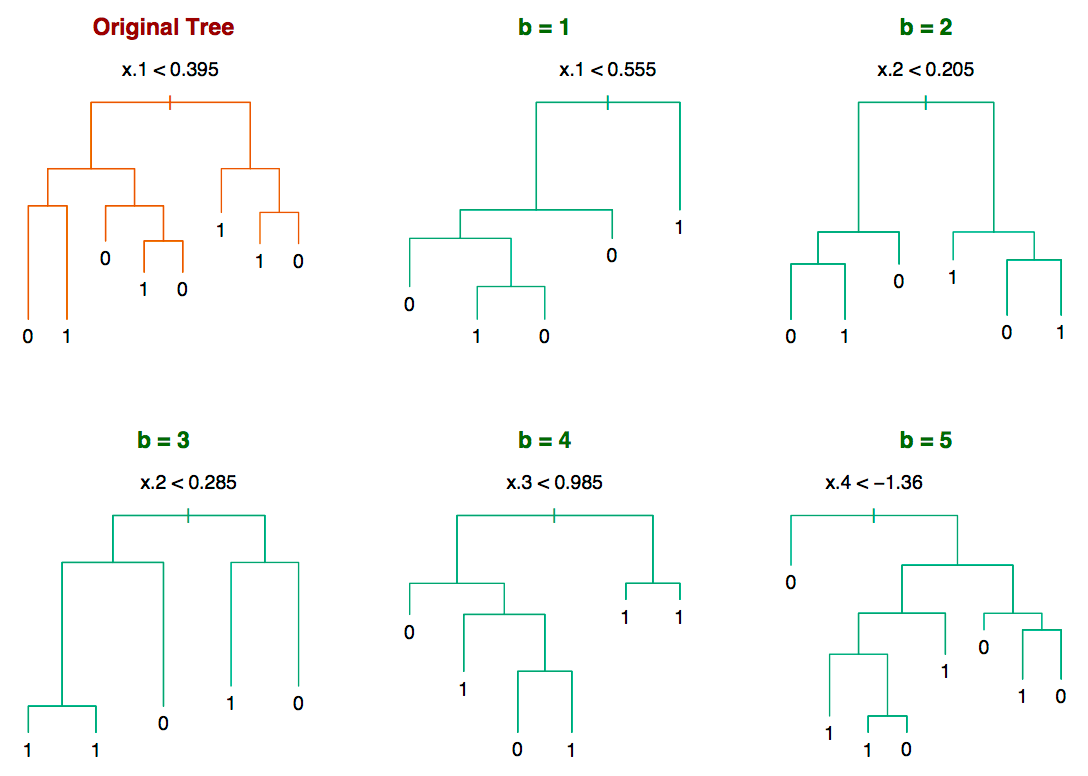
\includegraphics[width=1\columnwidth]{figures/baggedTrees}

\pause{}

\column{.6\textwidth}
\begin{itemize}[<+->]
\item Each bootstrap tree is quite different: different splitting variable at the root!

\item \textbf{High variance}: small perturbations of the training data lead to a high degree of model variability

\item Bagging helps most when the base learners are relatively unbiased but have high variance (exactly the case for
    decision trees)

\end{itemize}
\end{columns}

\end{itemize}
\let\thefootnote\relax\footnotetext{\tiny{From HTF Figure 8.9}}
\end{frame}
%

\subsection{Random Forests}
\begin{frame}{Motivating Random Forests: Correlated Prediction Functions}
Recall the motivating principle of bagging:
    \begin{itemize}[<+->]
\item For $\hat{\theta}_{1},\ldots,\hat{\theta}_{n}$ \emph{i.i.d.} with $\ex\pb{\hat{\theta}}=\theta$ and $\var\pb{\hat{\theta}}=\sigma^{2}$,
\[
\ex\left[\frac{1}{n}\sum_{i=1}^{n}\hat{\theta}_{i}\right]=\mu\qquad\var\left[\frac{1}{n}\sum_{i=1}^{n}\hat{\theta}_{i}\right]=\frac{\sigma^{2}}{n}.
\]

\item What if $\hat{\theta}$'s are correlated? 

%\item Suppose $\forall i\neq j$, $\text{Corr}(\hat{\theta}_{i},\hat{\theta}_{j})=\rho$ . Then
%\[
%\var\left[\frac{1}{n}\sum_{i=1}^{n}\hat{\theta}_{i}\right]=\rho\sigma^{2}+\frac{1-\rho}{n}\sigma^{2}.
%\]

\item For large $n$, the covariance term dominates, limiting the benefits of averaging
\item Bootstrap samples are 
\begin{itemize}
\item independent samples from the training set, but
\item \al{not} independent samples from $P_{\cx\times\cy}$
\end{itemize}

\item Can we reduce the dependence between $\hat{f}_{i}$'s?
\end{itemize}
\end{frame}

\begin{frame}{Random Forests}
\begin{simpleblock}{\textbf{Key idea}}
Use bagged decision trees, but modify the tree-growing procedure
to reduce the dependence between trees.
\end{simpleblock}

\begin{itemize}[<+->]
\item Build a collection of trees independently (in parallel), as before
\item When constructing each tree node, restrict choice of splitting
variable to a randomly chosen subset of features of size $m$
\begin{itemize}
    \item<.-> This prevents a situation where all trees are dominated by the same small number of strong features (and are therefore too similar to each other)
\end{itemize}
\item We typically choose $m\approx\sqrt{p}$, where $p$ is the number of
    features (or we can choose $m$ using cross validation)
\item If $m = p$, this is just bagging
\end{itemize}
\note[item]{When $m$ is too small, you might underfit. When $m$ is too large, it won't be effective at reducing dependence.}
\end{frame}
%
\begin{frame}{Random Forests: Effect of $m$} 
\begin{figure}
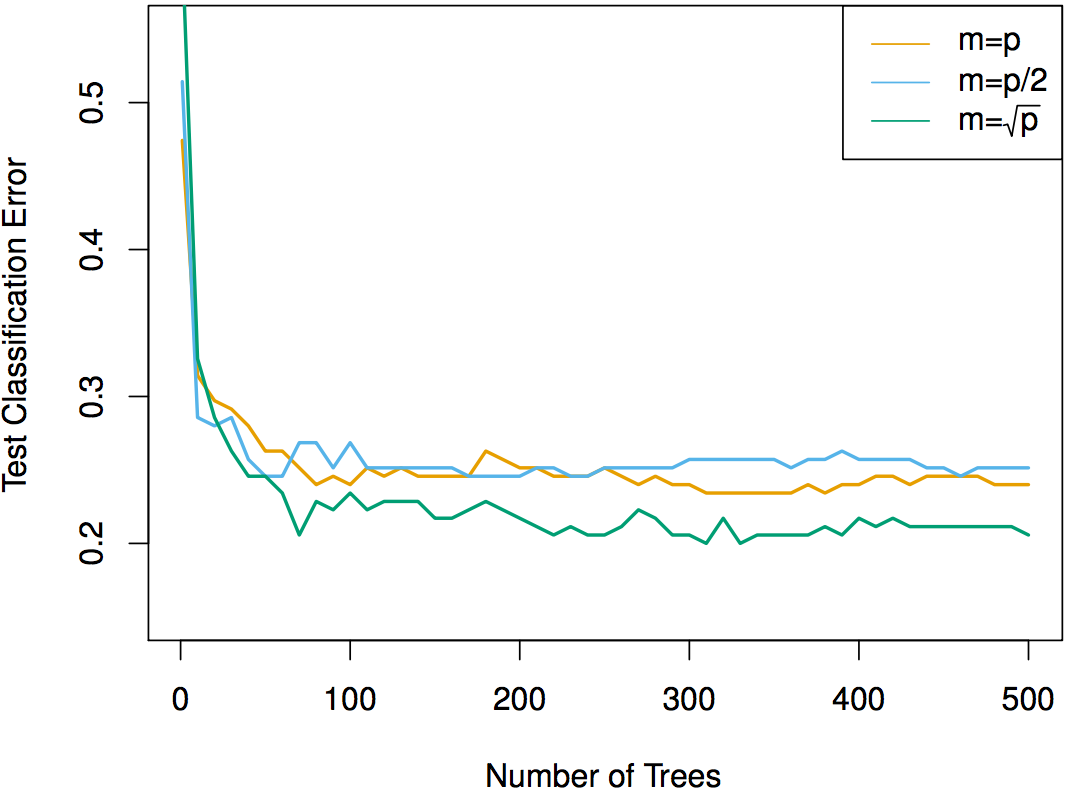
\includegraphics[height=0.7\textheight]{figures/randomForestVsBagging}
\end{figure}

\let\thefootnote\relax\footnotetext{\tiny{From \emph{An Introduction to Statistical Learning, with applications in R} (Springer, 2013) with permission from the authors: G. James, D. Witten,  T. Hastie and R. Tibshirani.}}
\end{frame}

\begin{frame}{Review}
\begin{itemize}[<+->]
\item The usual approach is to build very deep trees---low bias but \al{high variance}
\item Ensembling many models reduces variance
\begin{itemize}[<.->]
\item Motivation: Mean of i.i.d. estimates has smaller variance than single estimate
\end{itemize}
\item Use bootstrap to simulate many data samples from one dataset
\begin{itemize}[<.->]
\item $\implies$ Bagged decision trees
\end{itemize}
\item But bootstrap samples (and the induced models) are correlated
\item Ensembling works better when we combine a diverse set of
prediction functions
\begin{itemize}[<.->]
    \item $\implies$ Random forests: select a random subset of features for each decision tree
\end{itemize}
\end{itemize}
\end{frame}

\section{Boosting}
\begin{frame}
{Boosting: Overview}
\begin{description}[<+->]
    \item[Bagging] Reduce variance of a low bias, high variance estimator by ensembling many estimators trained in parallel (on different datasets obtained through sampling).
\item[Boosting] Reduce the error rate of a high bias estimator by ensembling many estimators trained in sequence (without bootstrapping).
\begin{itemize}
\item Like bagging, boosting is a general method that is particularly popular with decision trees.
\item Main intuition: instead of fitting the data very closely using a large decision tree, train gradually, using a sequence of simpler trees
\end{itemize}
\end{description}
\end{frame}

    \begin{frame}{Boosting: Overview}
        \begin{itemize}[<+->]
\item A \textbf{weak/base learner} is a classifier that does slightly better than chance.
\item<.-> Weak learners are like rules of thumb:
\begin{itemize}[<.->]
\item ``Inheritance'' $\implies$ spam
\item From a friend $\implies$ not spam
\end{itemize}
\item \textbf{Key idea}:
\begin{itemize}
\item Each weak learner focuses on different training examples (\emph{reweighted data})
\item Weak learners make different contributions to the final prediction (\emph{reweighted classifier})
\end{itemize}
        \item A set of smaller, simpler trees may improve interpretability
        \item We'll focus on a specific implementation, AdaBoost (Freund \& Schapire, 1997)
\end{itemize} 
\end{frame}

\subsection{Adaboost: The Algorithm}
\begin{frame}{AdaBoost: Setting}

\begin{itemize}[<+->]
\item Binary classification: $\cy=\left\{ -1,1\right\} $ 

\item {Base hypothesis space} $\ch=\left\{ h:\cx\to {\color{blue}\left\{ -1,1\right\}} \right\} $. 

\item Typical base hypothesis spaces:
\begin{itemize}[<.->]
\item \textbf{Decision stumps} (tree with a single split)
\item Trees with few terminal nodes
\item Linear decision functions
\end{itemize}
\end{itemize}
\end{frame}
%
\begin{frame}{Weighted Training Set}
Each base learner is trained on weighted data.
\begin{itemize}
\item Training set $\cd=\left(\left(x_{1},y_{1}\right),\ldots,\left(x_{n},y_{n}\right)\right)$.
\item Weights $\left(w_{1},\ldots,w_{n}\right)$ associated with each example.

\pause{}
\item \textbf{Weighted empirical risk}:
\[
\hat{R}_{n}^{w}(f)\eqdef \frac{1}{W}\sum_{i=1}^{n}w_{i}\ell\left(f(x_{i}),y_{i}\right)\quad\mbox{where}\;W=\sum_{i=1}^{n}w_{i}
\]

\item Examples with larger weights affect the loss more.

\end{itemize}
\end{frame}

\begin{frame}{AdaBoost: Schematic}
\begin{center}
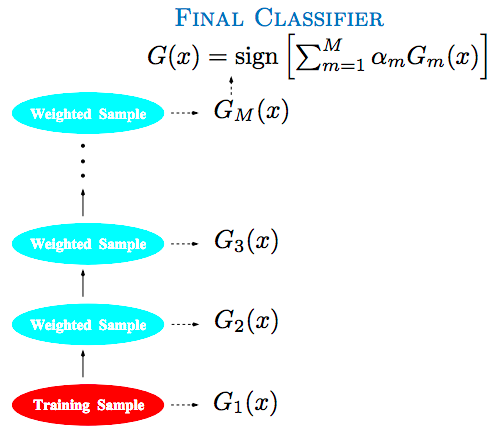
\includegraphics[height=0.7\textheight]{figures/adaboostSchematic}
\par\end{center}

\let\thefootnote\relax\footnotetext{\tiny{From ESL Figure 10.1}}
\end{frame}

\begin{frame}{AdaBoost: Sketch of the Algorithm}

\begin{itemize}[<+->]
%\item Training set $\cd=\left(\left(x_{1},y_{1}\right),\ldots,\left(x_{n},y_{n}\right)\right)$.
\item Start with equal weights for all training points: $w_{1}=\cdots=w_{n}=1$

\item Repeat for $m=1,\ldots,M$ (where $M$ is the number of classifiers we plan to train):

\begin{itemize}
\item Train base classifier $G_{m}(x)$ on the weighted training data; this classifier may not fit the data well

\item Increase the weight of the points misclassified by $G_{m}(x)$ (this is the key idea of boosting!)

\end{itemize}
%\item So far, we've generated $M$ classifiers: $G_{1},\ldots,G_{M}:\cx\to\left\{ -1,1\right\} $.
\item Our final prediction is $G(x)=\sign\left[\sum_{m=1}^{M}\alpha_{m}G_{m}(x)\right]$
\end{itemize}

\end{frame}

\begin{frame}{AdaBoost: Classifier Weights}
    \begin{itemize}
\item Our final prediction is $G(x)=\sign\left[\sum_{m=1}^{M}\alpha_{m}G_{m}(x)\right]$.
\item We would like $\alpha_{m}$ to be:
\begin{itemize}
\item Nonnegative
\item Larger when $G_{m}$ fits its weighted training data well
\end{itemize}
\item The \textbf{weighted 0-1 error} of $G_{m}(x)$ is
\[
\mbox{err}_{m}=\frac{1}{W}\sum_{i=1}^{n}w_{i}\ind{y_{i}\neq G_{m}(x_{i})}\quad\text{where }W=\sum_{i=1}^{n}w_{i}.
\]
\item $\text{err}_{m}\in[0,1]$
\end{itemize}
\end{frame}
%
\begin{frame}{AdaBoost: Classifier Weights}
\begin{itemize}
\item The weight of classifier $G_{m}(x)$ is $\alpha_{m}=\ln\left(\frac{1-\text{err}_{m}}{\text{err}_{m}}\right)$

\pause{}
\end{itemize}
\begin{center}
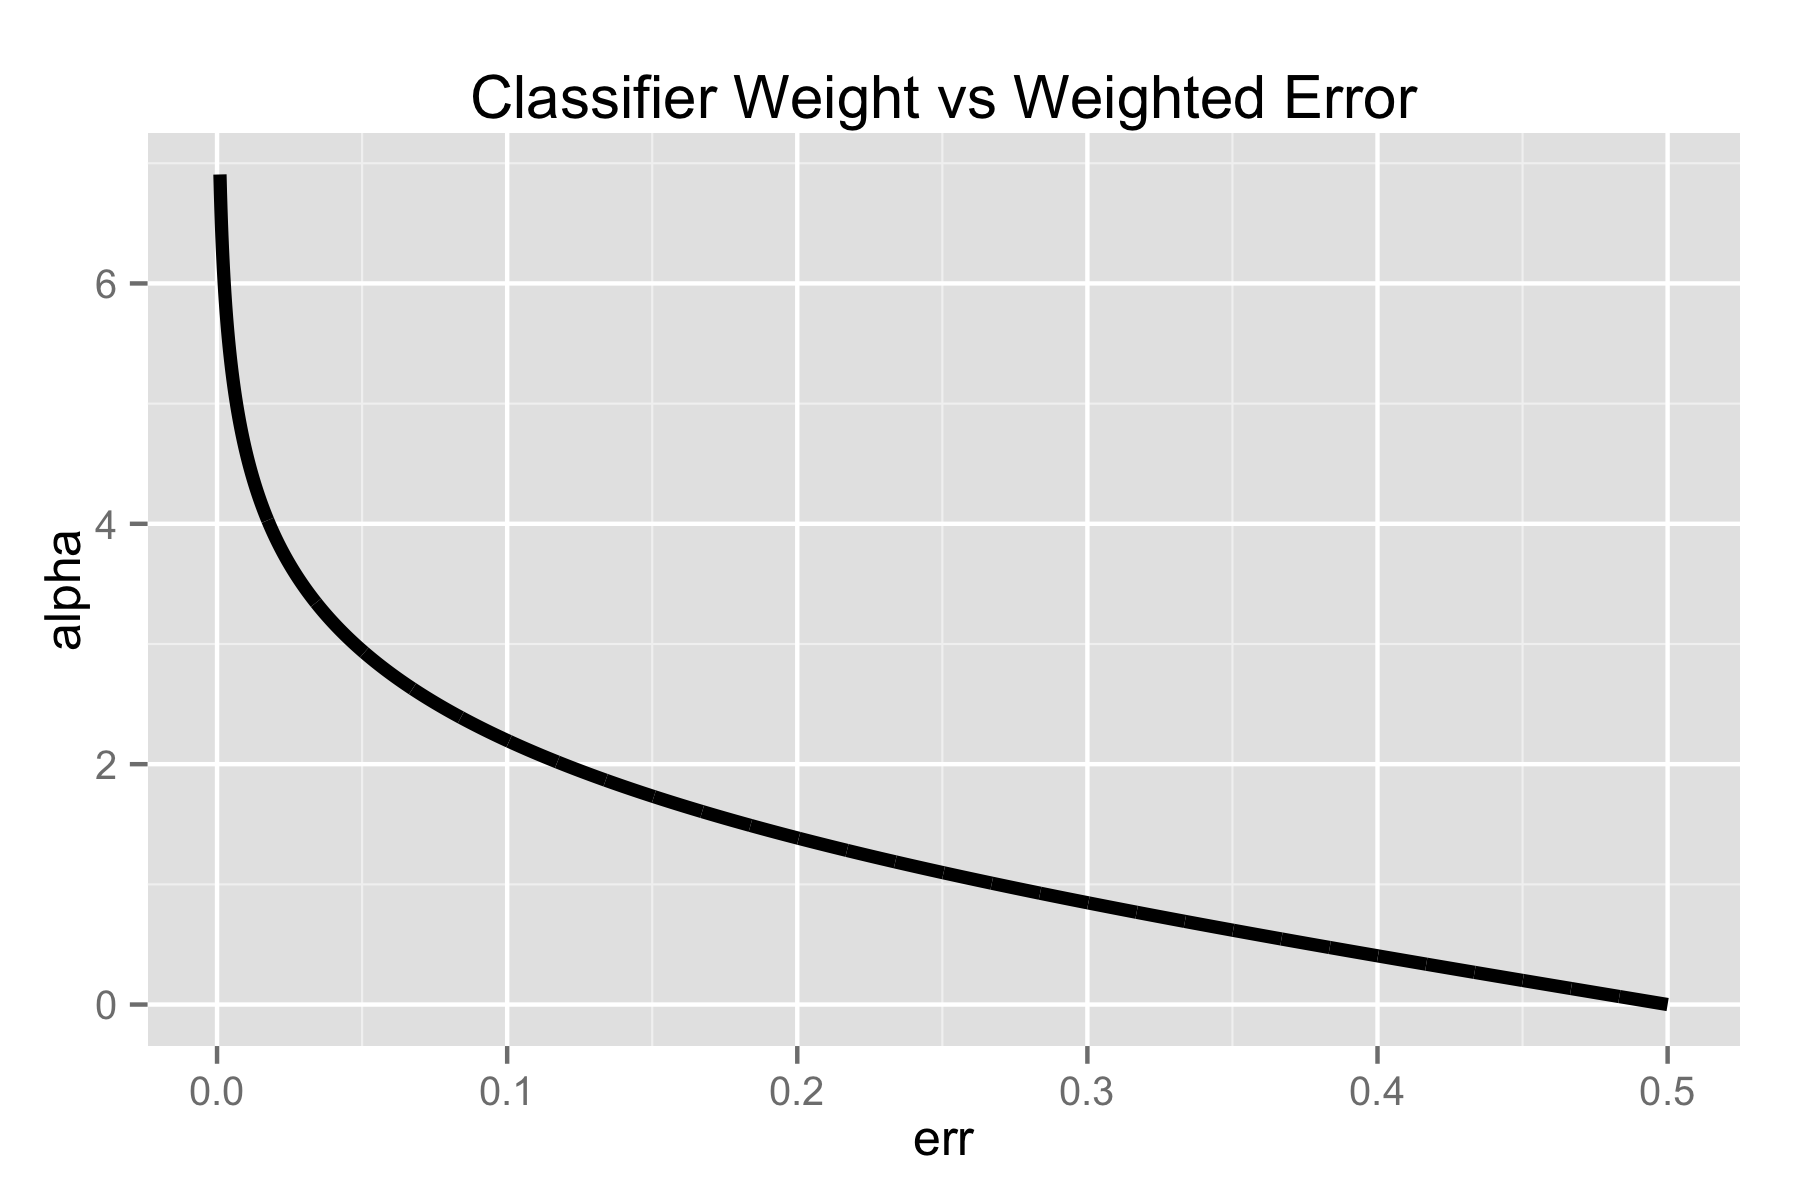
\includegraphics[clip,height=0.5\textheight]{figures/adaboostAlphaVsError}
\par\end{center}
\begin{itemize}
\item Higher weighted error $\implies$ lower weight
%\item When is $\alpha_m < 0$?
\end{itemize}

\end{frame}
%
\begin{frame}{Adaboost: Example Reweighting}
\begin{itemize}
    \item We train $G_{m}$ to minimize weighted error; the resulting error rate is $\text{err}_{m}$

\item<.-> Then $\alpha_{m}=\ln\left(\frac{1-\text{err}_{m}}{\text{err}_{m}}\right)$
is the weight of $G_{m}$ in the final ensemble
\end{itemize}

\onslide<+->{
We want the next base learner to focus more on examples misclassified by the previous learner.
}
\begin{itemize}[<+->]
\item Suppose $w_{i}$ is the weight of example $x_i$ before training:
\begin{itemize}
\item If $G_{m}$ classifies $x_{i}$ correctly, keep $w_{i}$ as is

\item Otherwise, increase $w_{i}$:
\begin{eqnarray*}
w_{i} & \gets & w_{i}e^{\alpha_{m}}\\
& = & w_{i}\left(\frac{1-\text{err}_{m}}{\text{err}_{m}}\right)
\end{eqnarray*}

\item If $G_m$ is a strong classifier overall, then its $\alpha_m$ will be large; this means that if $x_i$ is misclassified, $w_i$ will increase to a greater extent
%\item<.-> For $\mbox{err}_{m}<0.5$ (weak learner), this always increases the weight.
\end{itemize}
\end{itemize}
\end{frame}
%
%\begin{frame}{Adaboost: Example Reweighting}
%\begin{itemize}
%\item Any misclassified point has weight adjusted as $w_{i}\gets w_{i}\left(\frac{1-\text{err}_{m}}{\text{err}_{m}}\right)$.
%\end{itemize}
%\begin{center}
%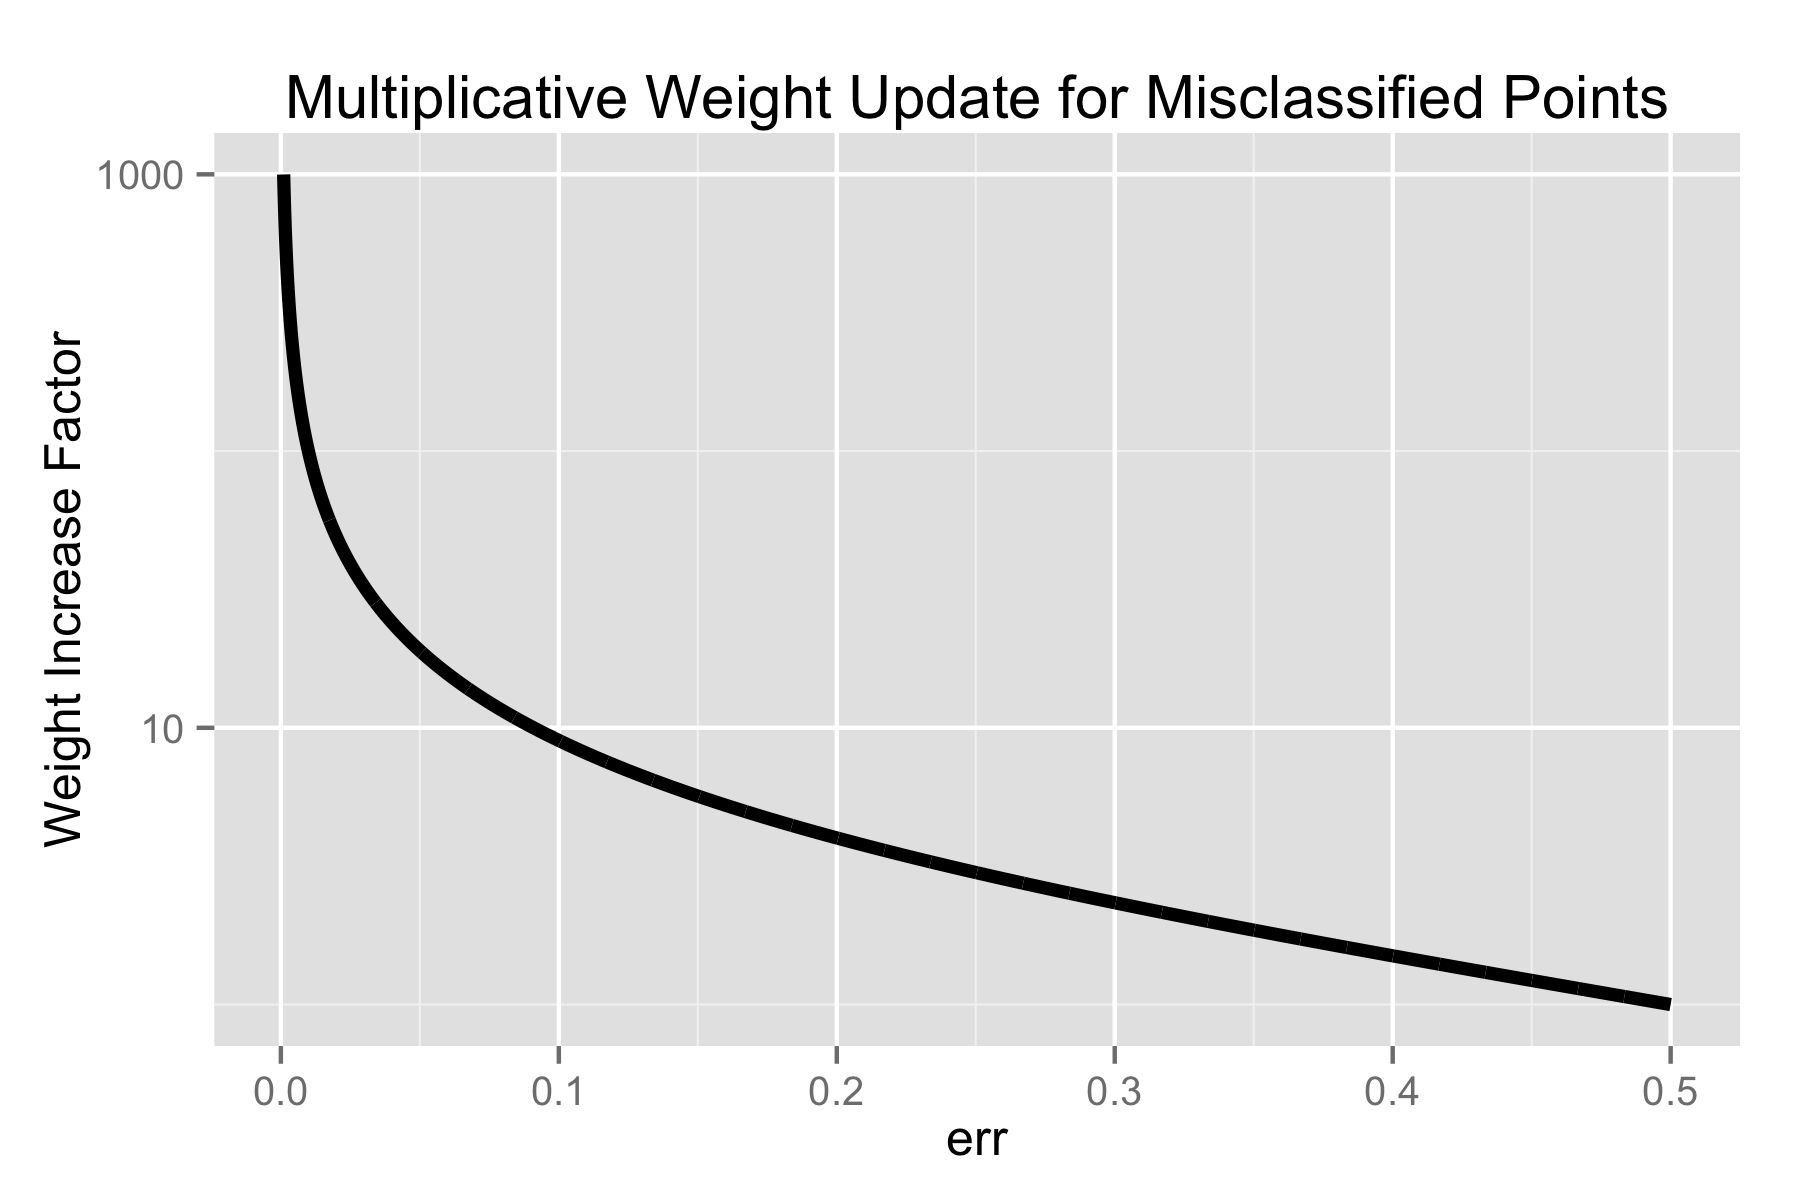
\includegraphics[clip,height=0.6\textheight]{figures/adaboostWeightUpdate}
%\par\end{center}
%\begin{itemize}
%\item The smaller $\err_{m}$, the more we increase weight of misclassified
%points.
%\end{itemize}
%\end{frame}
%
%\begin{frame}{AdaBoost: Algorithm}

%Given training set $\cd=\left\{ \left(x_{1},y_{1}\right),\ldots,\left(x_{n},y_{n}\right)\right\} $.
%\begin{enumerate}
%\item Initialize observation weights $w_{i}=1$, $i=1,2,\ldots,n$.

%\pause{}
%\item For $m=1$ to $M$:
%\begin{enumerate}
%\item Base learner fits weighted training data and returns $G_{m}(x)$

%\pause{}
%\item Compute \emph{weighted empirical 0-1 risk}:
%\[
%\mbox{err}_{m}=\frac{1}{W}\sum_{i=1}^{n}w_{i}\ind{y_{i}\neq G_{m}(x_{i})}\quad\text{where }W=\sum_{i=1}^{n}w_{i}.
%\]


%\pause{}
%\item Compute  \emph{classifier weight}: $\alpha_{m}=\ln\left(\frac{1-\text{err}_{m}}{\text{err}_{m}}\right)$.

%\pause{}
%\item Update \emph{example weight}: $w_{i}\gets w_{i}\cdot\exp\left[\alpha_{m}\ind{y_{i}\neq G_{m}(x_{i})}\right]$

%\pause{}
%\end{enumerate}
%\item Return \emph{voted classifier}: $G(x)=\sign\left[\sum_{m=1}^{M}\alpha_{m}G_{m}(x)\right]$.
%\end{enumerate}
%\end{frame}
%
\begin{frame}{AdaBoost with Decision Stumps}
\begin{itemize}
\item After 1 round:
\end{itemize}
\begin{figure}
\begin{centering}
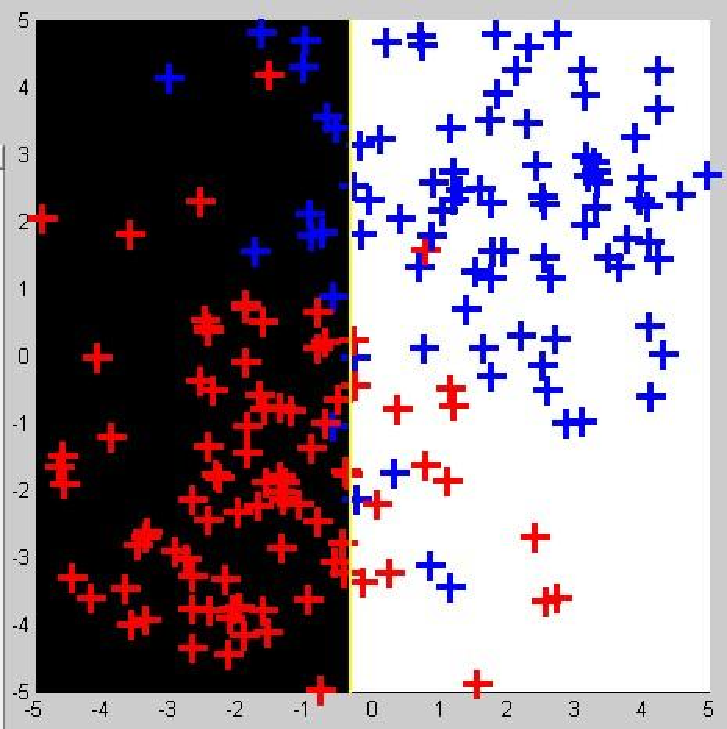
\includegraphics[height=0.5\textheight]{{figures/fig16.10a}.pdf}
\par\end{centering}
\caption{{\footnotesize{}Size of plus sign represents weight of example. Blackness represents preference for red class; whiteness represents preference for blue class.}}
\end{figure}

\let\thefootnote\relax\footnotetext{\tiny{KPM Figure 16.10}}
\end{frame}
%
\begin{frame}{AdaBoost with Decision Stumps}
\begin{itemize}
\item After 3 rounds:
\end{itemize}
\begin{figure}
\begin{centering}
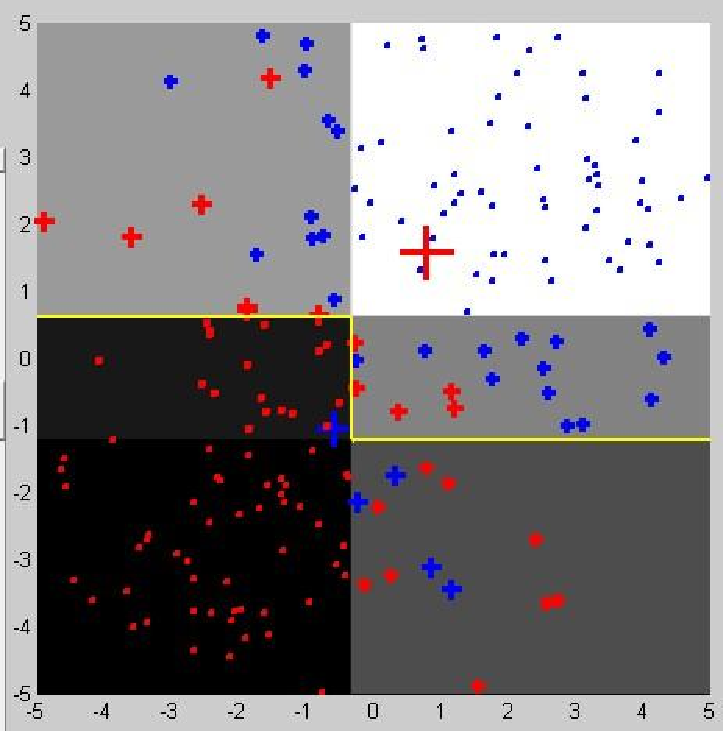
\includegraphics[clip,height=0.5\textheight]{{figures/fig16.10b}.pdf}
\par\end{centering}
\caption{{\footnotesize{}Size of plus sign represents weight of example. Blackness represents preference for red class; whiteness represents preference for blue class.}}
\end{figure}

\let\thefootnote\relax\footnotetext{\tiny{KPM Figure 16.10}}
\end{frame}
%
\begin{frame}{AdaBoost with Decision Stumps}
\begin{itemize}
\item After 120 rounds:
\end{itemize}
\begin{figure}
\begin{centering}
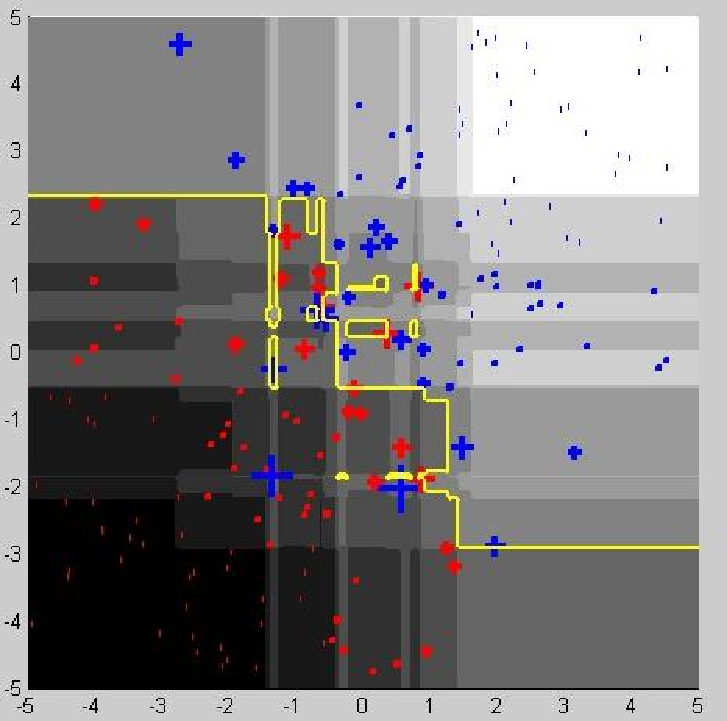
\includegraphics[height=0.5\textheight]{{figures/fig16.10c}.pdf}
\par\end{centering}
\caption{{\footnotesize{}Size of plus sign represents weight of example. Blackness represents preference for red class; whiteness represents preference for blue class.}}
\end{figure}

\let\thefootnote\relax\footnotetext{\tiny{KPM Figure 16.10}}
\end{frame}

\begin{frame}{Does AdaBoost overfit?}
\begin{itemize}
\item Does a large number of rounds of boosting lead to overfitting?
\item If we were overfitting, the learning curves would look like:
\end{itemize}
\begin{center}
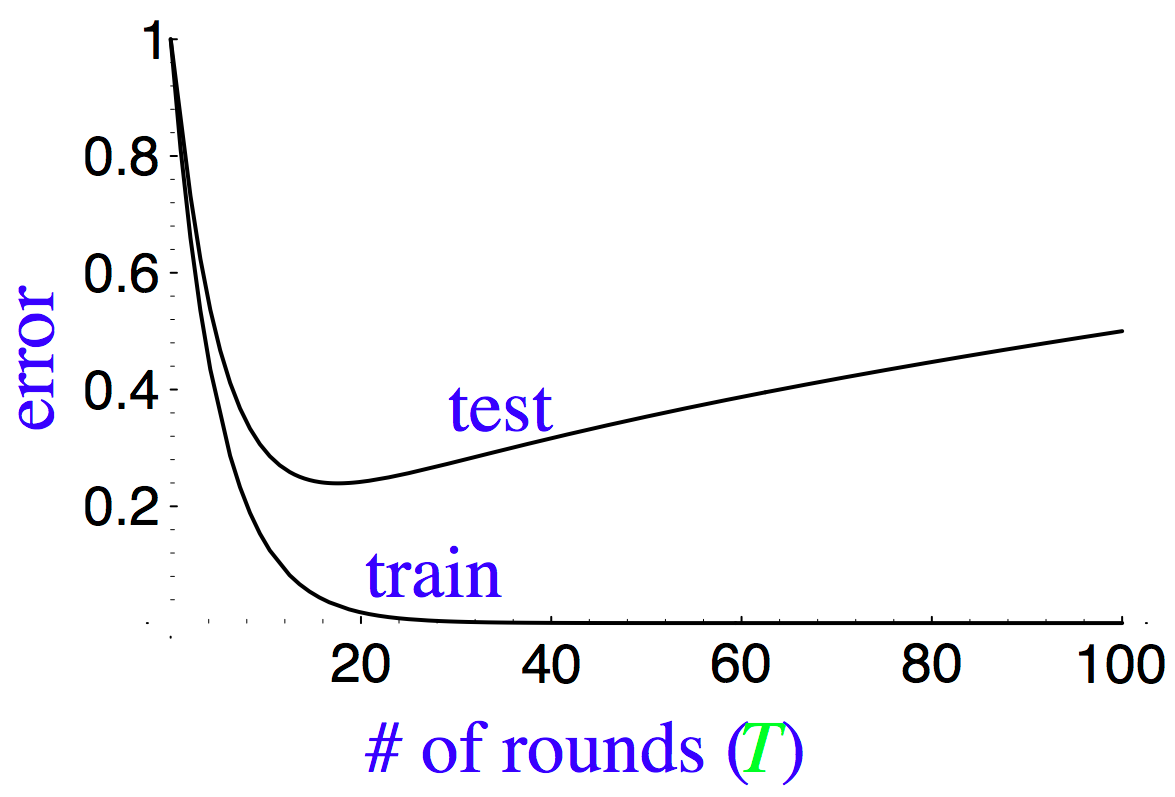
\includegraphics[height=0.55\textheight]{figures/typicalTrainTestCurve}
\par\end{center}

\let\thefootnote\relax\footnotetext{\tiny{From Rob Schapire's NIPS 2007 Boosting tutorial.}}
\end{frame}
%
\begin{frame}{Learning Curves for AdaBoost}
\begin{itemize}
\item AdaBoost is usually quite resistant to overfitting
\item The test error continues to decrease even after the training error drops to zero!
\end{itemize}
\begin{center}
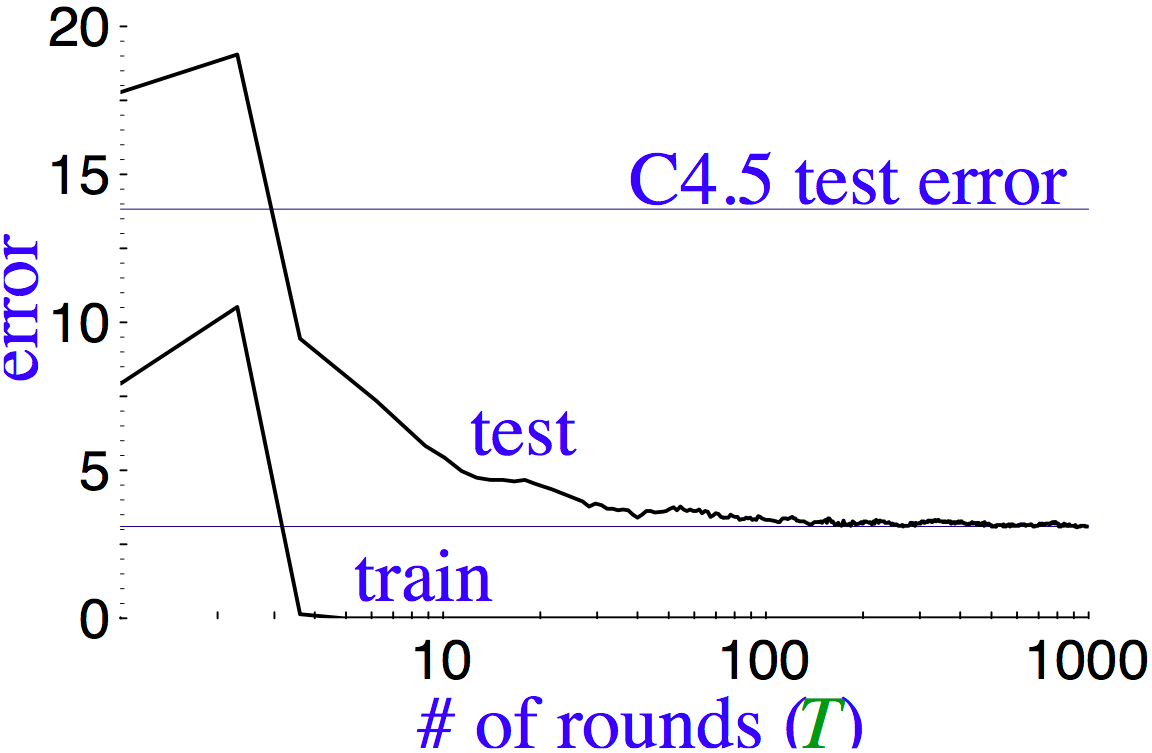
\includegraphics[height=0.55\textheight]{figures/actualTrainTestCurves}
\par\end{center}

\let\thefootnote\relax\footnotetext{\tiny{From Rob Schapire's NIPS 2007 Boosting tutorial.}}
\end{frame}


\begin{frame}
{Summary}
    \begin{itemize}[<+->]
\item Boosting is used to reduce bias from shallow decision trees
\item AdaBoost is a very powerful off-the-self classifier!
\item Next week
\begin{itemize}
\item What is the objective function of AdaBoost?
\item Generalizations to other loss functions 
\end{itemize}
\end{itemize}
\end{frame}

\end{document}
